Całość oprogramowania wykorzystuje język programowania \texttt{C++}. Projektowana oraz implementowana sieć składa się
z~dwóch typów modułów, stąd też pojawiła się potrzeba zainicjowania dwóch osobnych projektów -- jednego pod elementy
sieci LoRa oraz drugiego, dedykowanego dla modułu serwera sieciowego (ang. \textsl{webserver}), z~uwagi na zupełnie inną
platformę sprzętową. Firmware napisany został z~wykorzystaniem kilku różnych podejść:
\begin{itemize}[label=--]
    \item modułowego: każdy plik źródłowy odpowiada za zbiór funkcji wykonujących określone zadania (np. praca
          z~biblioteką do modułów LoRa zaimplementowana jest w~pliku \texttt{lora.cpp}),
    \item obiektowego: większość elementów kodu źródłowego jest reprezentowana w~postaci osobnego obiektu. Każdy
          z~nich posiada swoje funkcje oraz pełni określone zadania (np. obiekt \enquote{\texttt{bme}} ma za zadanie
          umożliwić współpracę z~sensorami dostępnymi na płytce czujników BME280, która podłączona jest do każdego
          modułu SLAVE).
\end{itemize}
Ponadto, wykorzystane zostały elementy języka \texttt{C++}, które dostępne są w~nowszych wersjach -- funkcje szablonowe
(ang. \textsl{template functions}) lub pętle typu \texttt{for-range}. Są to elementy, które znacznie ułatwiły
implementację kodu oraz pozwoliły na minimalizację powtarzalności pewnych elementów.

Z~uwagi na zastosowanie podejścia modułowego, całość oprogramowania składa się z~wielu mniejszych elementów,
podzielonych na odpowiadające im pliki. Aby mieć pewność, że implementowane funkcje nie będą posiadały żadnych kolizji
w~swoich nazwach zastosowane zostały przestrzenie nazw (ang. \textsl{namespaces}). Dodatkowo, ponieważ kod źródłowy
jest dostępny w~domenie publicznej (repozytorium na platformie GitHub z~licencją \textsl{MIT} \cite{snyk-sw-license}),
podjęta została decyzja o~dodaniu opisów działania do wszystkich elementów. Wykorzystany został do tego \textsl{Doxygen}
-- narzędzie do generowania dokumentacji (np. formie strony internetowej lub dokumentu w~\LaTeX) na podstawie
specjalnych znaczników w~komentarzach \cite{doxygen}.

\FloatBarrier
\section{Framework oraz biblioteki\label{sect:framework-libraries}} Bazą do oprogramowania na wszystkich modułach jest
framework Arduino oraz jego modyfikacja pod platformę STM32 -- stm32duino, która pozwala na wykorzystanie pełnej
funkcjonalności rdzenia Arduino \cite{stm32duino-docs}. Pomimo tego, że biblioteki HAL (ang. \textsl{Hardware
    Abstraction Layer}) oraz framework STM32 są narzędziami dedykowanymi, w~przypadku tego projektu nie można było ich
zastosować. Oryginalna biblioteka do obsługi modułów rozszerzeń LoRa została wycofana z~użytku na rzecz nowszej
implementacji, pod nowszą wersję płytek Nucleo z~wbudowanym hardware.

\FloatBarrier
\subsection{Wykorzystane biblioteki\label{sect:used-libs}} Do implementacji oprogramowania na wszystkie moduły
wykorzystanych zostało kilka bibliotek, które pozwalały na dodanie pełnego zakresu funkcjonalności do każdego
z~projektów.

W~przypadku bibliotek zewnętrznych (niebędących częścią rdzenia Arduino) były to:
\begin{itemize}[label=--]
    \item STM32duino I-NUCLEO-LRWAN1: biblioteka do uruchomienia oraz pracy z~modułem rozszerzeń LoRa. Pozwala ona na
          pracę w~dwóch trybach: LoRaRadio -- implementacja wykorzystująca tylko standard dolnej warstwy sprzętowej LoRa
          oraz LoRaWAN -- dodająca możliwość podłączenia modułów do istniejącej sieci LoRa oraz wysyłanie i~odbieranie
          z~niej wiadomości,
    \item Adafruit BME280 Library: biblioteka dedykowana do modułów BME280, pozwalająca na zbieranie danych z~sensorów,
          wykorzystując do tego magistralę SPI albo I2C (w~zależności od posiadanego modułu rozszerzeń),
    \item Adafruit BusIO: uniwersalna biblioteka dodająca pewien poziom abstrakcji do komunikacji po magistralach I2C
          oraz SPI,
    \item WiFi101: biblioteka, która daje możliwość wykorzystania modułu WiFi obecnego na płytce Adafruit Feather M0
          (wykorzystanej do uruchomienia serwera w~sieci lokalnej).
\end{itemize}
Ponadto, wykorzystane zostały biblioteki I2C oraz SPI, dostępne w~rdzeniu Arduino. Potrzebne były one do uzyskania
komunikacji pomiędzy mikrokontrolerem Adafruit Feather M0 a~modułem WiFi, sensorami BM280 podłączonymi do modułów SLAVE
oraz do stworzenia połączenia pomiędzy modułem MASTER a~płytką z~serwerem sieci lokalnej.

\FloatBarrier
\subsection{Ograniczenia związane z~wykorzystaniem Arduino oraz STM32duino\label{sect:framework-limits}} STM32duino,
pomimo tego, że ułatwił, bądź w~ogóle pozwolił na pracowanie z~wykorzystywanymi modułami, nie jest platformą idealną,
pozbawioną ograniczeń. Jedynym z~nich, które w~dość znacznym stopniu utrudniło implementację oprogramowania dla modułów
sieci, był brak przerwań programowych oraz ograniczone możliwości zastosowania przerwań sprzętowych. Stąd też pojawił
się wymóg zastosowania pewnych obejść, jednocześnie tracąc na wydajności implementowanego rozwiązania. Ponadto,
występowały też problemy związane z~działaniem magistrali I2C, tutaj w~przypadku modułów Feather oraz standardowego
Arduino -- niemożliwe było wykorzystanie wyświetlacza OLED pracującego na magistrali I2C oraz zarejestrowania samego
mikrokontrolera jako części, z~którą można komunikować się po tej magistrali.

\FloatBarrier
\section{Implementacja oprogramowania elementów sieci\label{sect:firmware-network}} Zaprojektowana sieć składała się
w~sumie z~pięciu modułów -- 4~z~nich stanowiły elementy sieci LoRa, natomiast ostatni był wykorzystywany jako serwer
w~sieci lokalnej. W~projekcie nie została wykorzystana pełna funkcjonalność LoRaWAN oraz typowa dla niej architektura
(przedstawiona w~sekcji \ref{sect:lorawan}, rys. \ref{img:lorawan-architecture}), ponieważ implementacja takiego
rozwiązania jest bardzo kosztowna i~wymaga znacznie większej ilości elementów. Aby móc skorzystać ze specyfikacji
wymagane jest posiadanie bramy (ang. \textsl{gateway}) oraz serwerów odpowiedzialnych za przyłączanie urządzeń,
zarządzanie siecią oraz serwera aplikacyjnego. Z~uwagi na to zastosowana została dużo prostsza i~mniej wymagająca metoda
budowania sieci, opierająca się na wykorzystaniu modułów w~formie nadajników radiowych, pracujących w~standardzie LoRa.
Schemat ideowy budowanej sieci przedstawiony został na rys. \ref{img:network-schematic}.

\begin{figure}[!htbp]
    \centering
    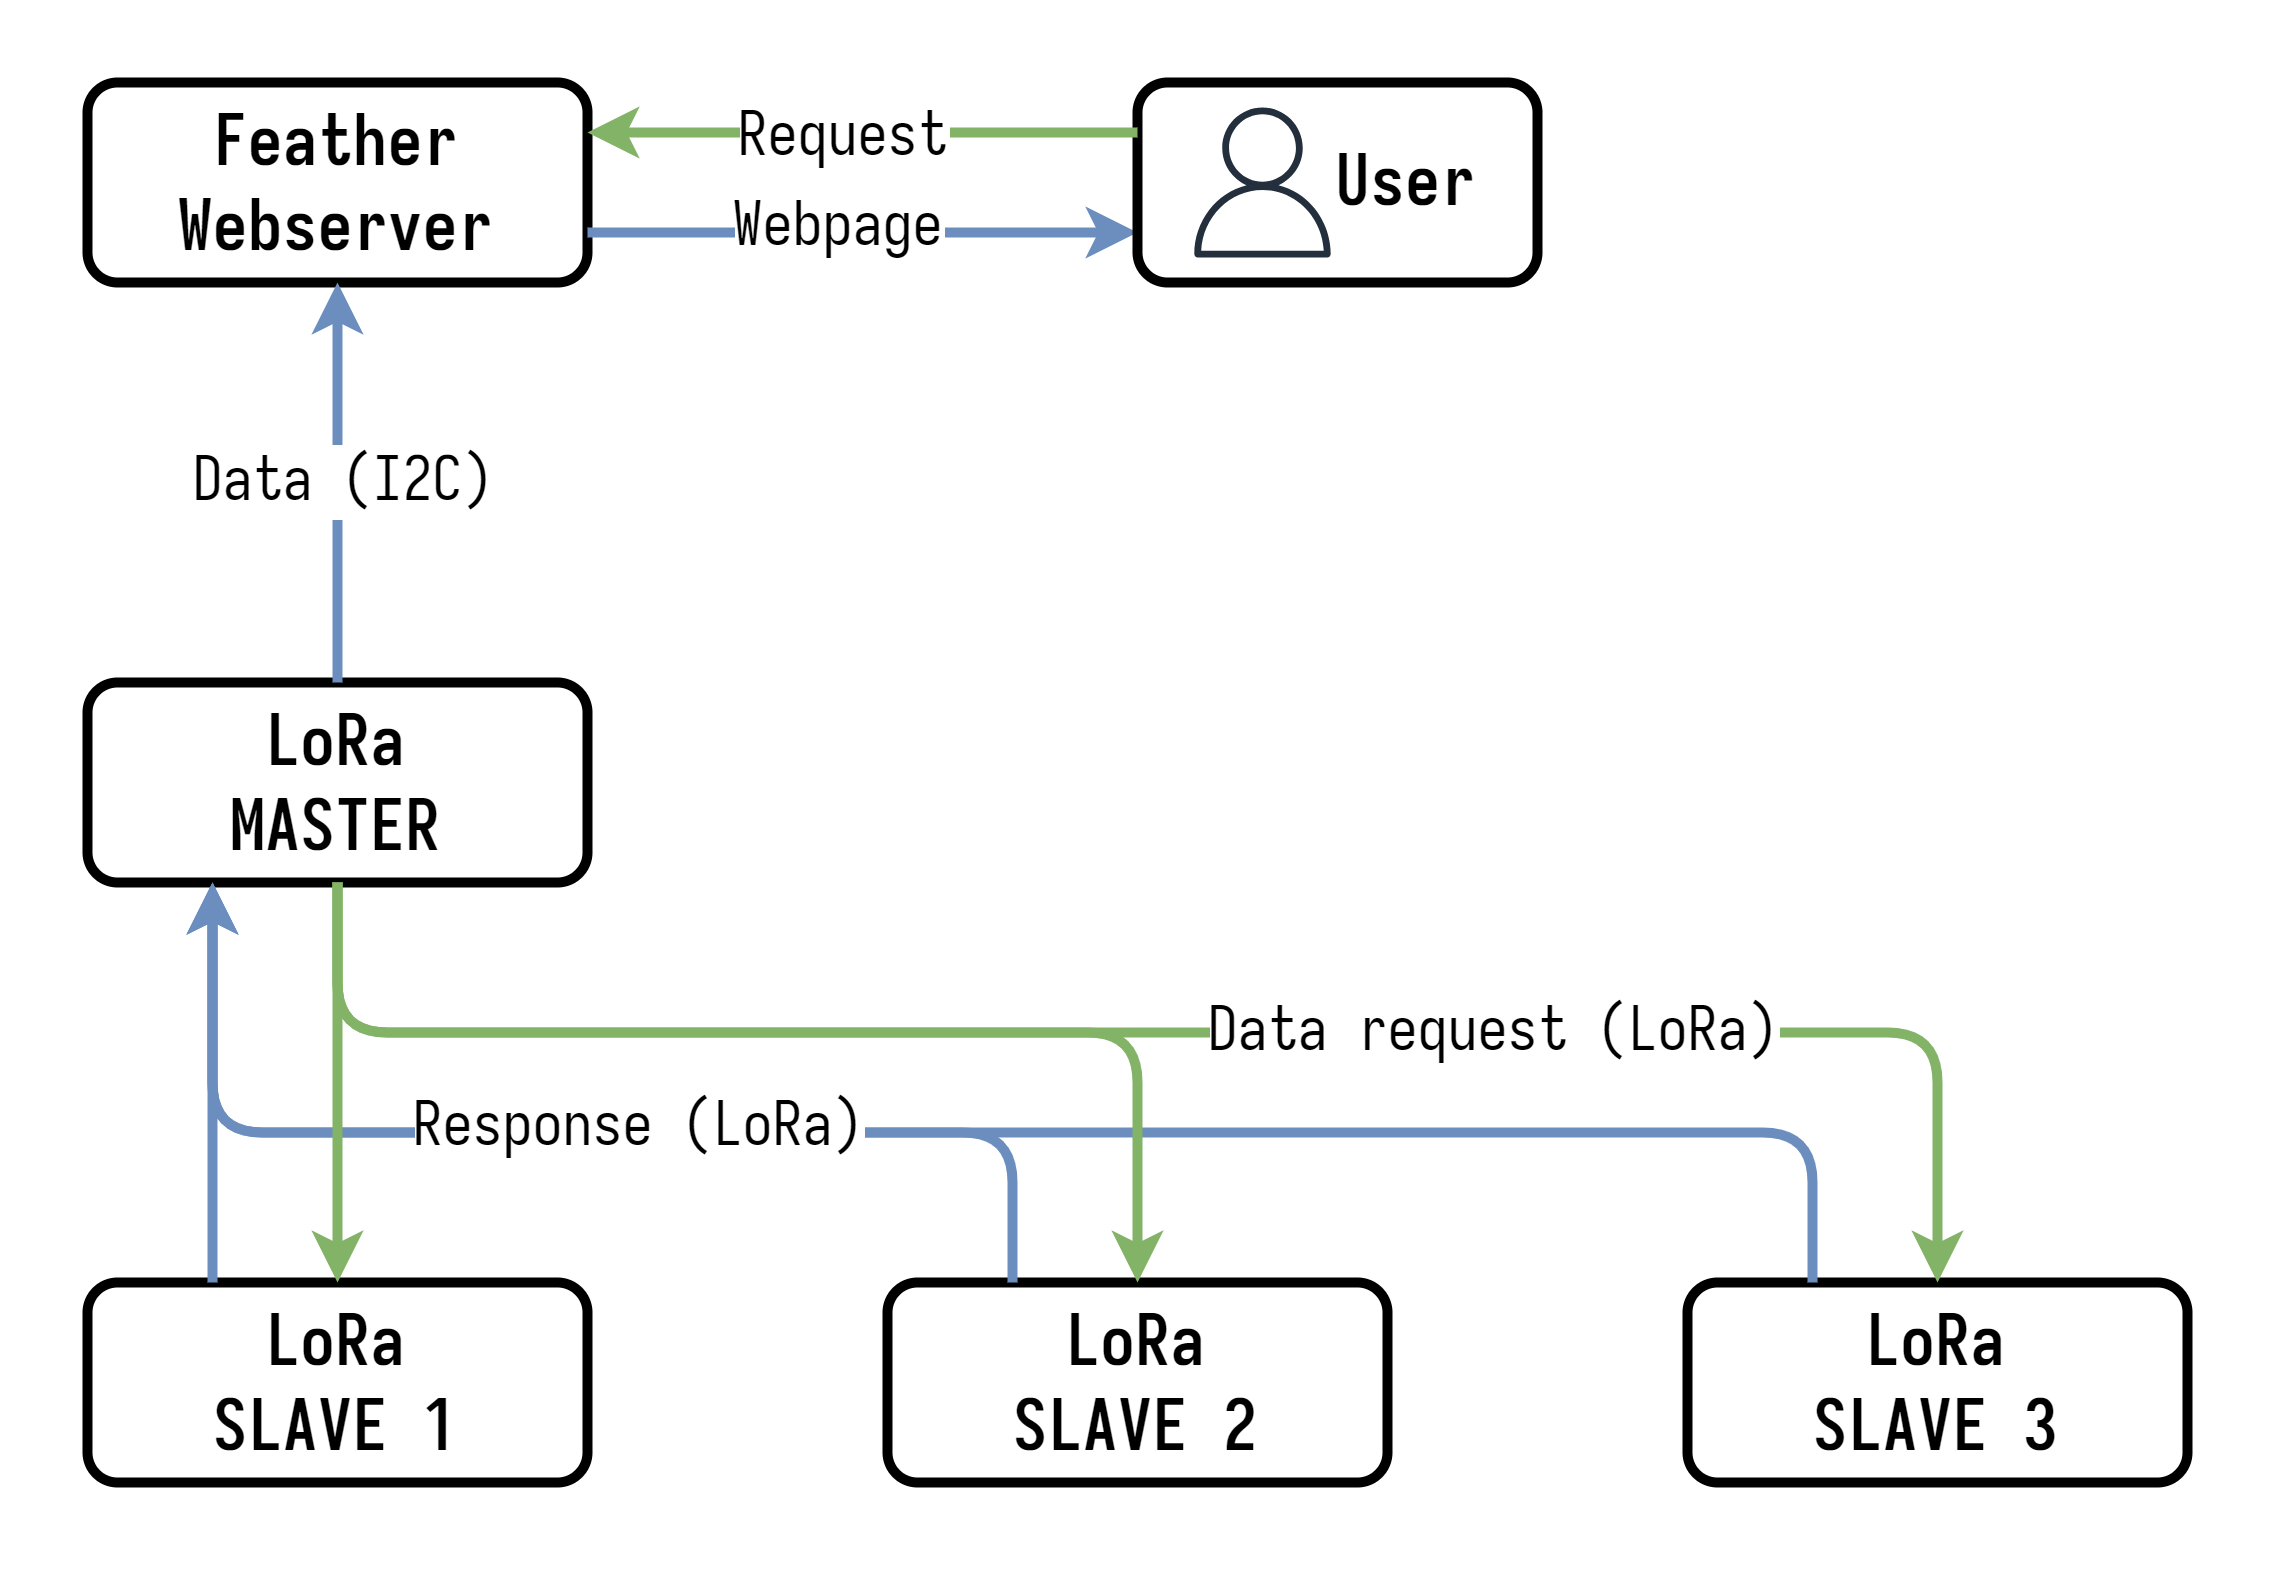
\includegraphics[width=0.8\textwidth]{lora-psn/images/network-schematic}
    \caption{\label{img:network-schematic}Schemat zbudowanej sieci, z~oznaczonymi elementami komunikacji}
\end{figure}

Oprogramowanie dla modułów pracujących w~sieci LoRa zostało zaimplementowane w~formie uniwersalnej -- jeden projekt
zawiera elementy dla modułu MASTER oraz modułów SLAVE. Plik konfiguracyjny projektu zawiera flagę, która definiuje, na
jaki typ modułu kod zostanie skompilowany. Co więcej, w~przypadku modułów SLAVE dodana została też flaga informująca
o~tym, jakie ID przypisane zostaje danej płytce. Rozwiązanie to odgrywa znaczącą rolę w~tym, jak wiadomości są
przesyłane w~sieci. Fragment pliku konfiguracyjnego, który odpowiedzialny jest za definiowanie tych elementów
przedstawiony został na listingu \ref{lst:lora-ini}.

\lstinputlisting[
    linerange={26-30},
    caption={Fragment pliku konfiguracyjnego (tutaj dla SLAVE1) odpowiedzialny za definicję typu oraz ID modułu},
    label={lst:lora-ini},
    float=htbp,
]{lora-psn/platformio.ini}

Wykorzystanie frameworku Arduino wymagało zastosowania pewnych schematów podczas implementacji. Dlatego też całość kodu
podzielona jest na dwie sekcje \texttt{setup()} oraz \texttt{loop()}, wykonywane odpowiednio raz, podczas startu modułu
oraz w~nieskończonej pętli, dopóki płytka ma zasilanie. Na rys. \ref{img:firmware-flowchart} przedstawiony został
schemat blokowy zaimplementowanego oprogramowania -- części zawartej w~sekcji \texttt{setup()}.

\begin{figure}[!htb]
    \centering
    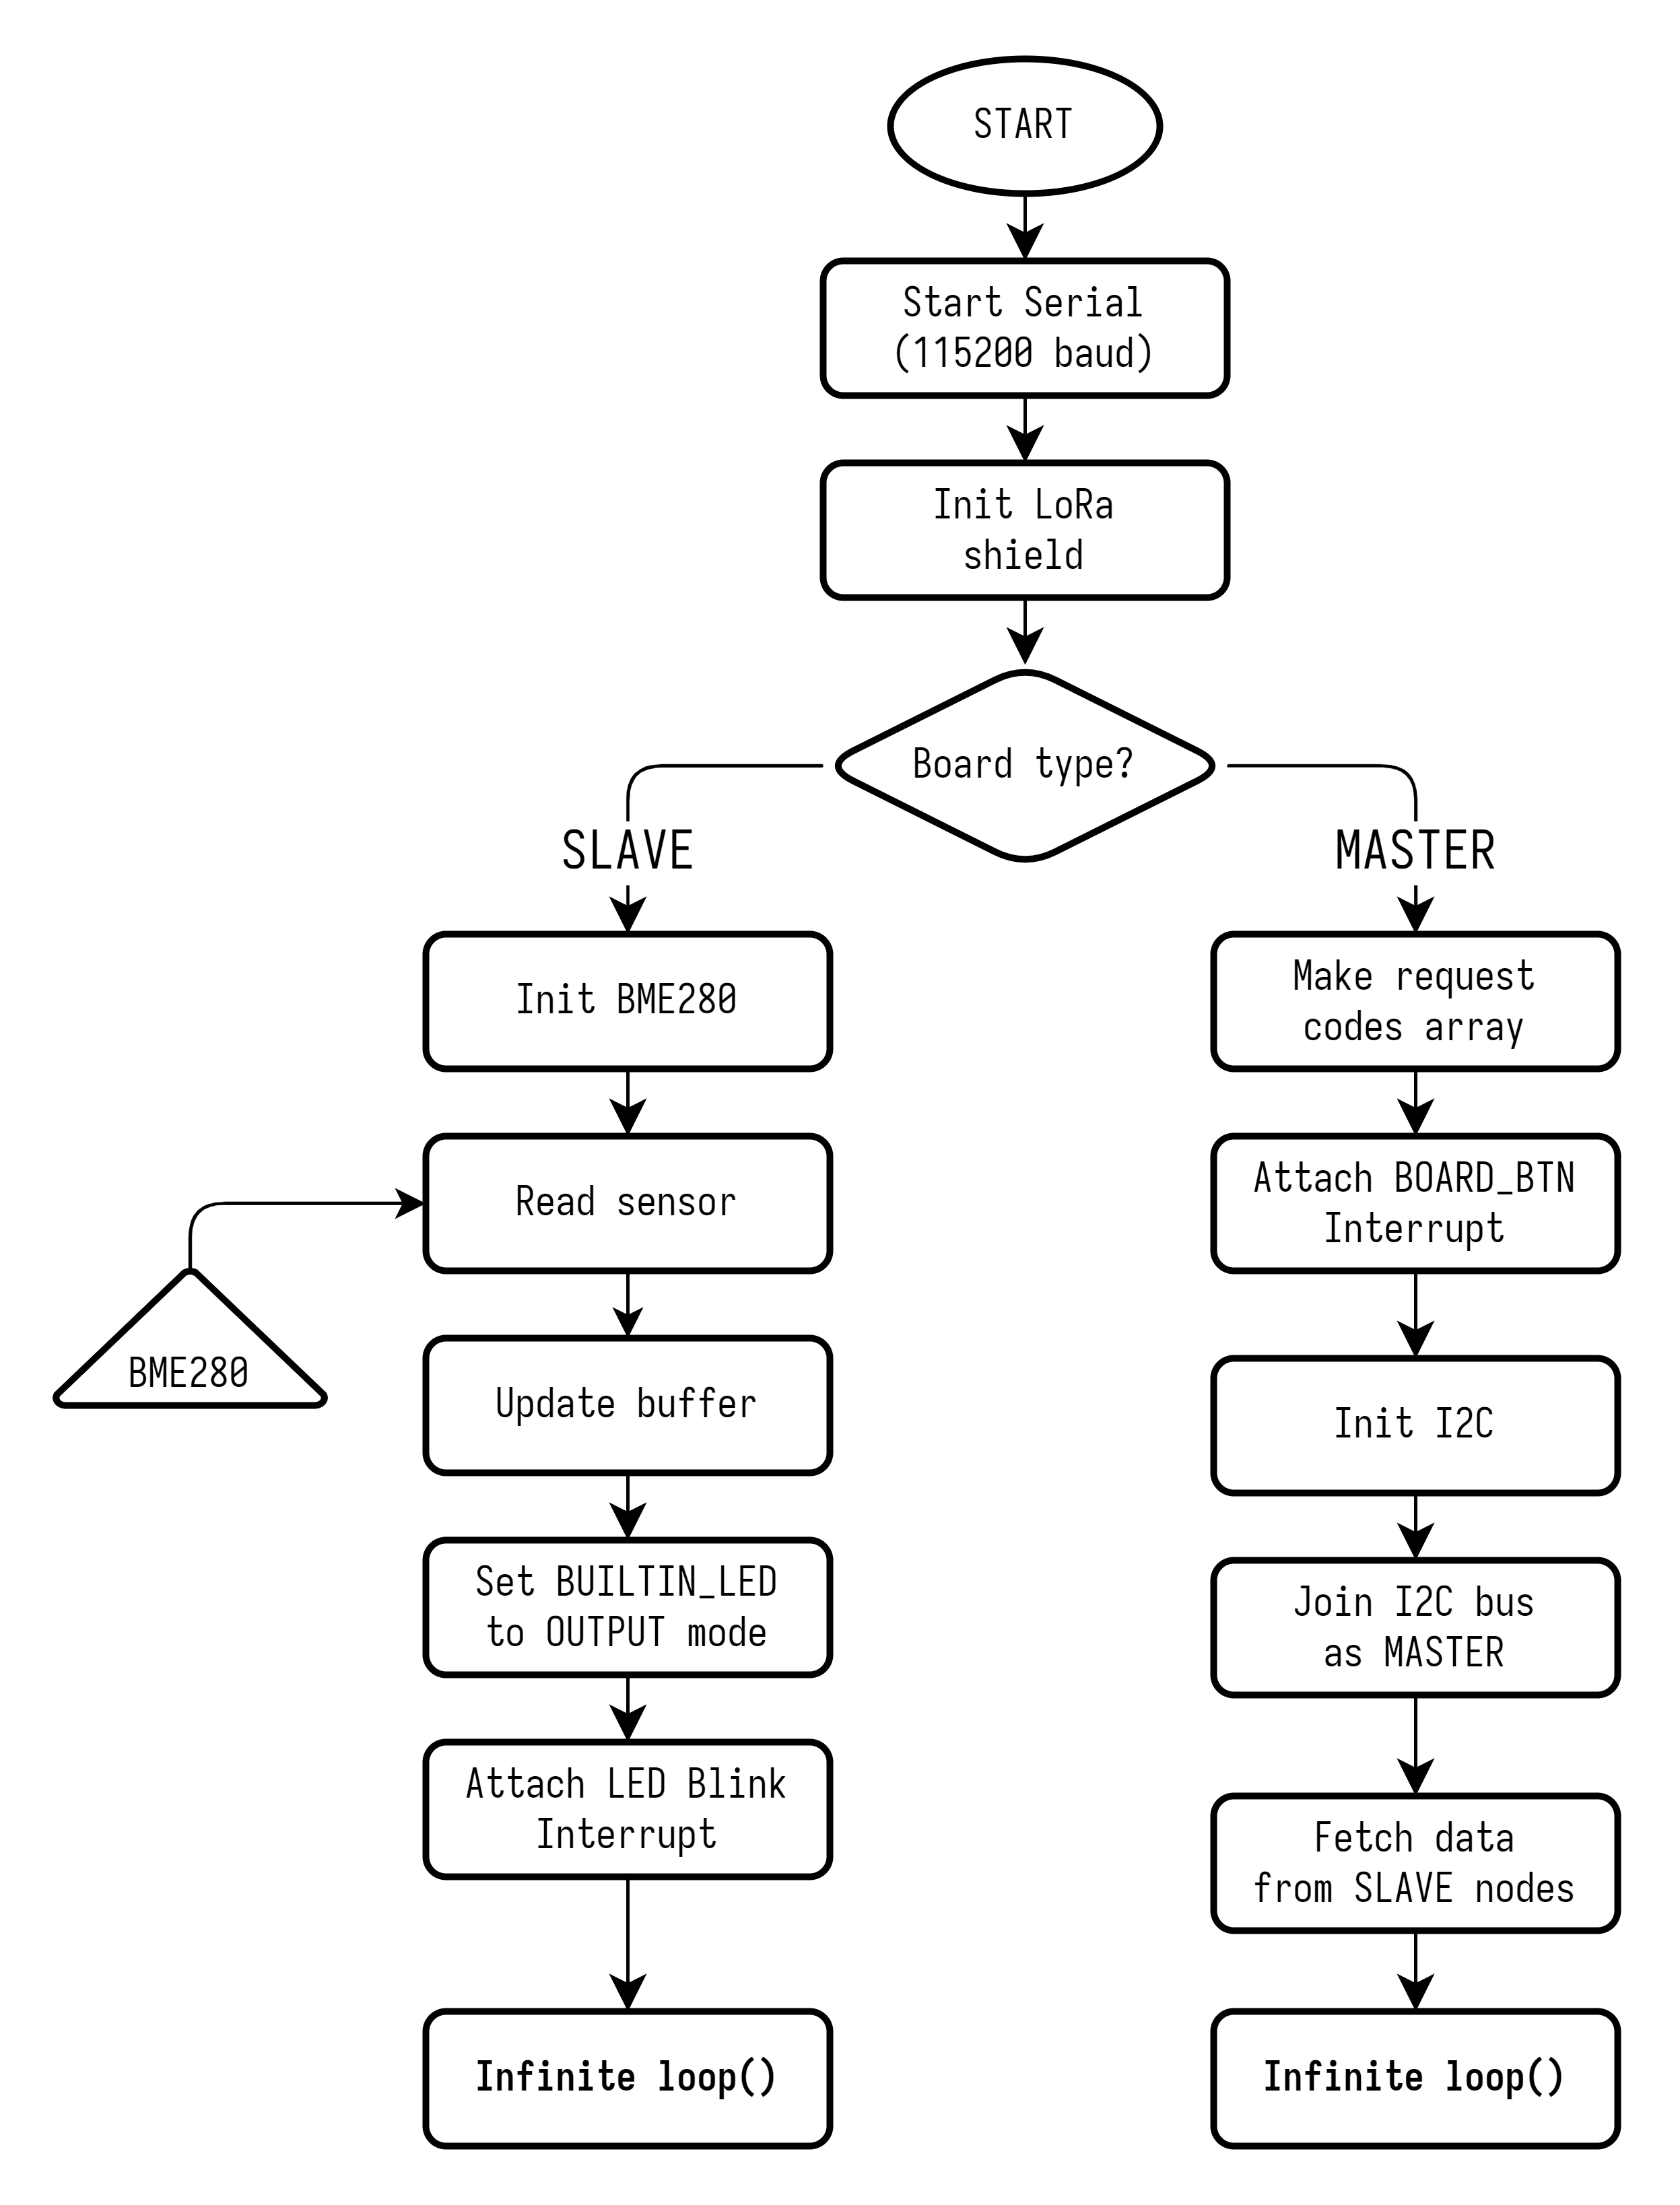
\includegraphics[width=0.9\textwidth]{lora-psn/images/firmware-flowchart}
    \caption{\label{img:firmware-flowchart}Schemat blokowy części \texttt{setup()} oprogramowania modułów sieci LoRa,
        z~podziałem na typ płytki}
\end{figure}

Oba typy oprogramowania zaczynają od ustawienia portu szeregowego na 115200 baud (szybkość transmisji), następnie
inicjowane jest rozszerzenie LoRa. Logowana jest informacja o~typie płytki, a~następnie kod oczekuje na informacje
o~starcie modułu rozszerzenia. W~przypadku błędu oraz poprawnego startu na port szeregowy wystawiana jest odpowiednia
informacja.

Następnie, w~zależności od typu płytki, wykonywane jest kilka operacji. W~przypadku modułów SLAVE są to:
\begin{enumerate}
    \item przygotowanie sensora BME280 oraz pobranie z~niego danych,
    \item aktualizacja zawartości bufora (wykorzystywanego do przechowywania odczytanych wartości),
    \item przygotowanie diody LED, która informuje o~trwającej komunikacji w~sieci,
    \item przygotowanie przerwania, wykorzystywanego do obsługi nowych zapytań.
\end{enumerate}

Natomiast dla modułów MASTER wykonywany jest inny zestaw operacji, z~uwagi na to, że taki moduł pełni zupełnie inną
funkcję w~sieci:
\begin{enumerate}
    \item przygotowanie tablicy z \enquote{kodami} zapytań (jedno bajtowe wartości do określenia czego żąda MASTER),
    \item inicjacja magistrali I2C i~podłączenie modułu jako MASTER,
    \item wykonanie podprogramu wysyłającego zapytania oraz odbierającego odpowiedzi od SLAVE-ów, tak aby tuż po
          starcie można było odczytać dane z~sieci.
\end{enumerate}
Ostatnim krokiem w~obu przypadkach jest przejście do nieskończonej pętli i~wykonywanie instrukcji w~niej zawartych,
wykorzystując do tego określony okres zegara.

Dodatkowo, oprogramowanie posiada zestaw definicji oraz funkcji wykorzystywanych do debugowania, które ułatwiały
implementację oprogramowania -- \texttt{globals.h} oraz \texttt{debug.h}. Najważniejszymi elementami pliku globalnych
definicji są funkcje preprocesora -- zwracających tylko ID modułu lub ID danej na podstawie kodu zapytania oraz
struktury szablonowe (ang. \textsl{template structures}), które zawierają informację o~tym jaki kształt powinny mieć
dane zbierane z~sensorów oraz przekazywane przez sieć. Definicję przedstawiono na listingu \ref{lst:globals}, natomiast
dla funkcji wysłającej sformatowane wiadomości przez port szeregowy na listingu \ref{lst:debug}. Implementacja oparta
została o~funkcję z~rdzeniu Arduino -- \texttt{Serial.println()}.

\lstinputlisting[
    language=C++,
    linerange={6-8,15-39},
    caption={Definicje funkcji dla preprocesora oraz struktury szablonowe (z polami o~jednej wartości oraz z~tablicami)},
    label={lst:globals},
    float=htbp,
]{lora-psn/include/globals.h}

\lstinputlisting[
    language=C++,
    linerange={20-26},
    caption={Funkcji wykorzystywana do wysyłania sformatowanych wiadomości przez port szeregowy},
    label={lst:debug},
    float=htbp,
]{lora-psn/include/debug.h}

\FloatBarrier
\subsection{Oprogramowanie modułu MASTER\label{sect:firmware-master}} Po wykonaniu instrukcji, które
opisane zostały w~poprzedniej sekcji, moduł MASTER przechodzi do pracy w~nieskończonej pętli -- \texttt{loop()}.
Wszystko oparte jest na zegarze o~zdefiniowanym okresie -- wybrana została wartość 1~minuty (60000 milisekund).
Implementacja oparta została o~zegar nieblokujący (ang. \textsl{non-blocking timer}) z~wykorzystaniem funkcji
\texttt{millis()} -- funkcji zwracającej ilość milisekund od momentu startu programu. Okres został zdefiniowany
w~definicjach preprocesora, w~celu uniknięcia tzw. magicznych liczb (ang. \textsl{magic numbers}).

W~momencie, gdy mija wymagany czas, program przechodzi do wykonania podprogramu odpowiadającego za wysyłanie zapytań
oraz zbieranie odpowiedzi z~sieci. Na rys. \ref{img:master-flowchart} przedstawiony został diagram blokowy instrukcji
wykonywanych przez moduł MASTER w~nieskończonej pętli oraz tego, co wykonywane jest w~podprogramie komunikacji.
Natomiast pełna implementacja obu tych elementów przedstawiona została na listingach \ref{lst:main-loop} oraz
\ref{lst:master-fetch}.

\begin{figure}[!htbp]
    \centering
    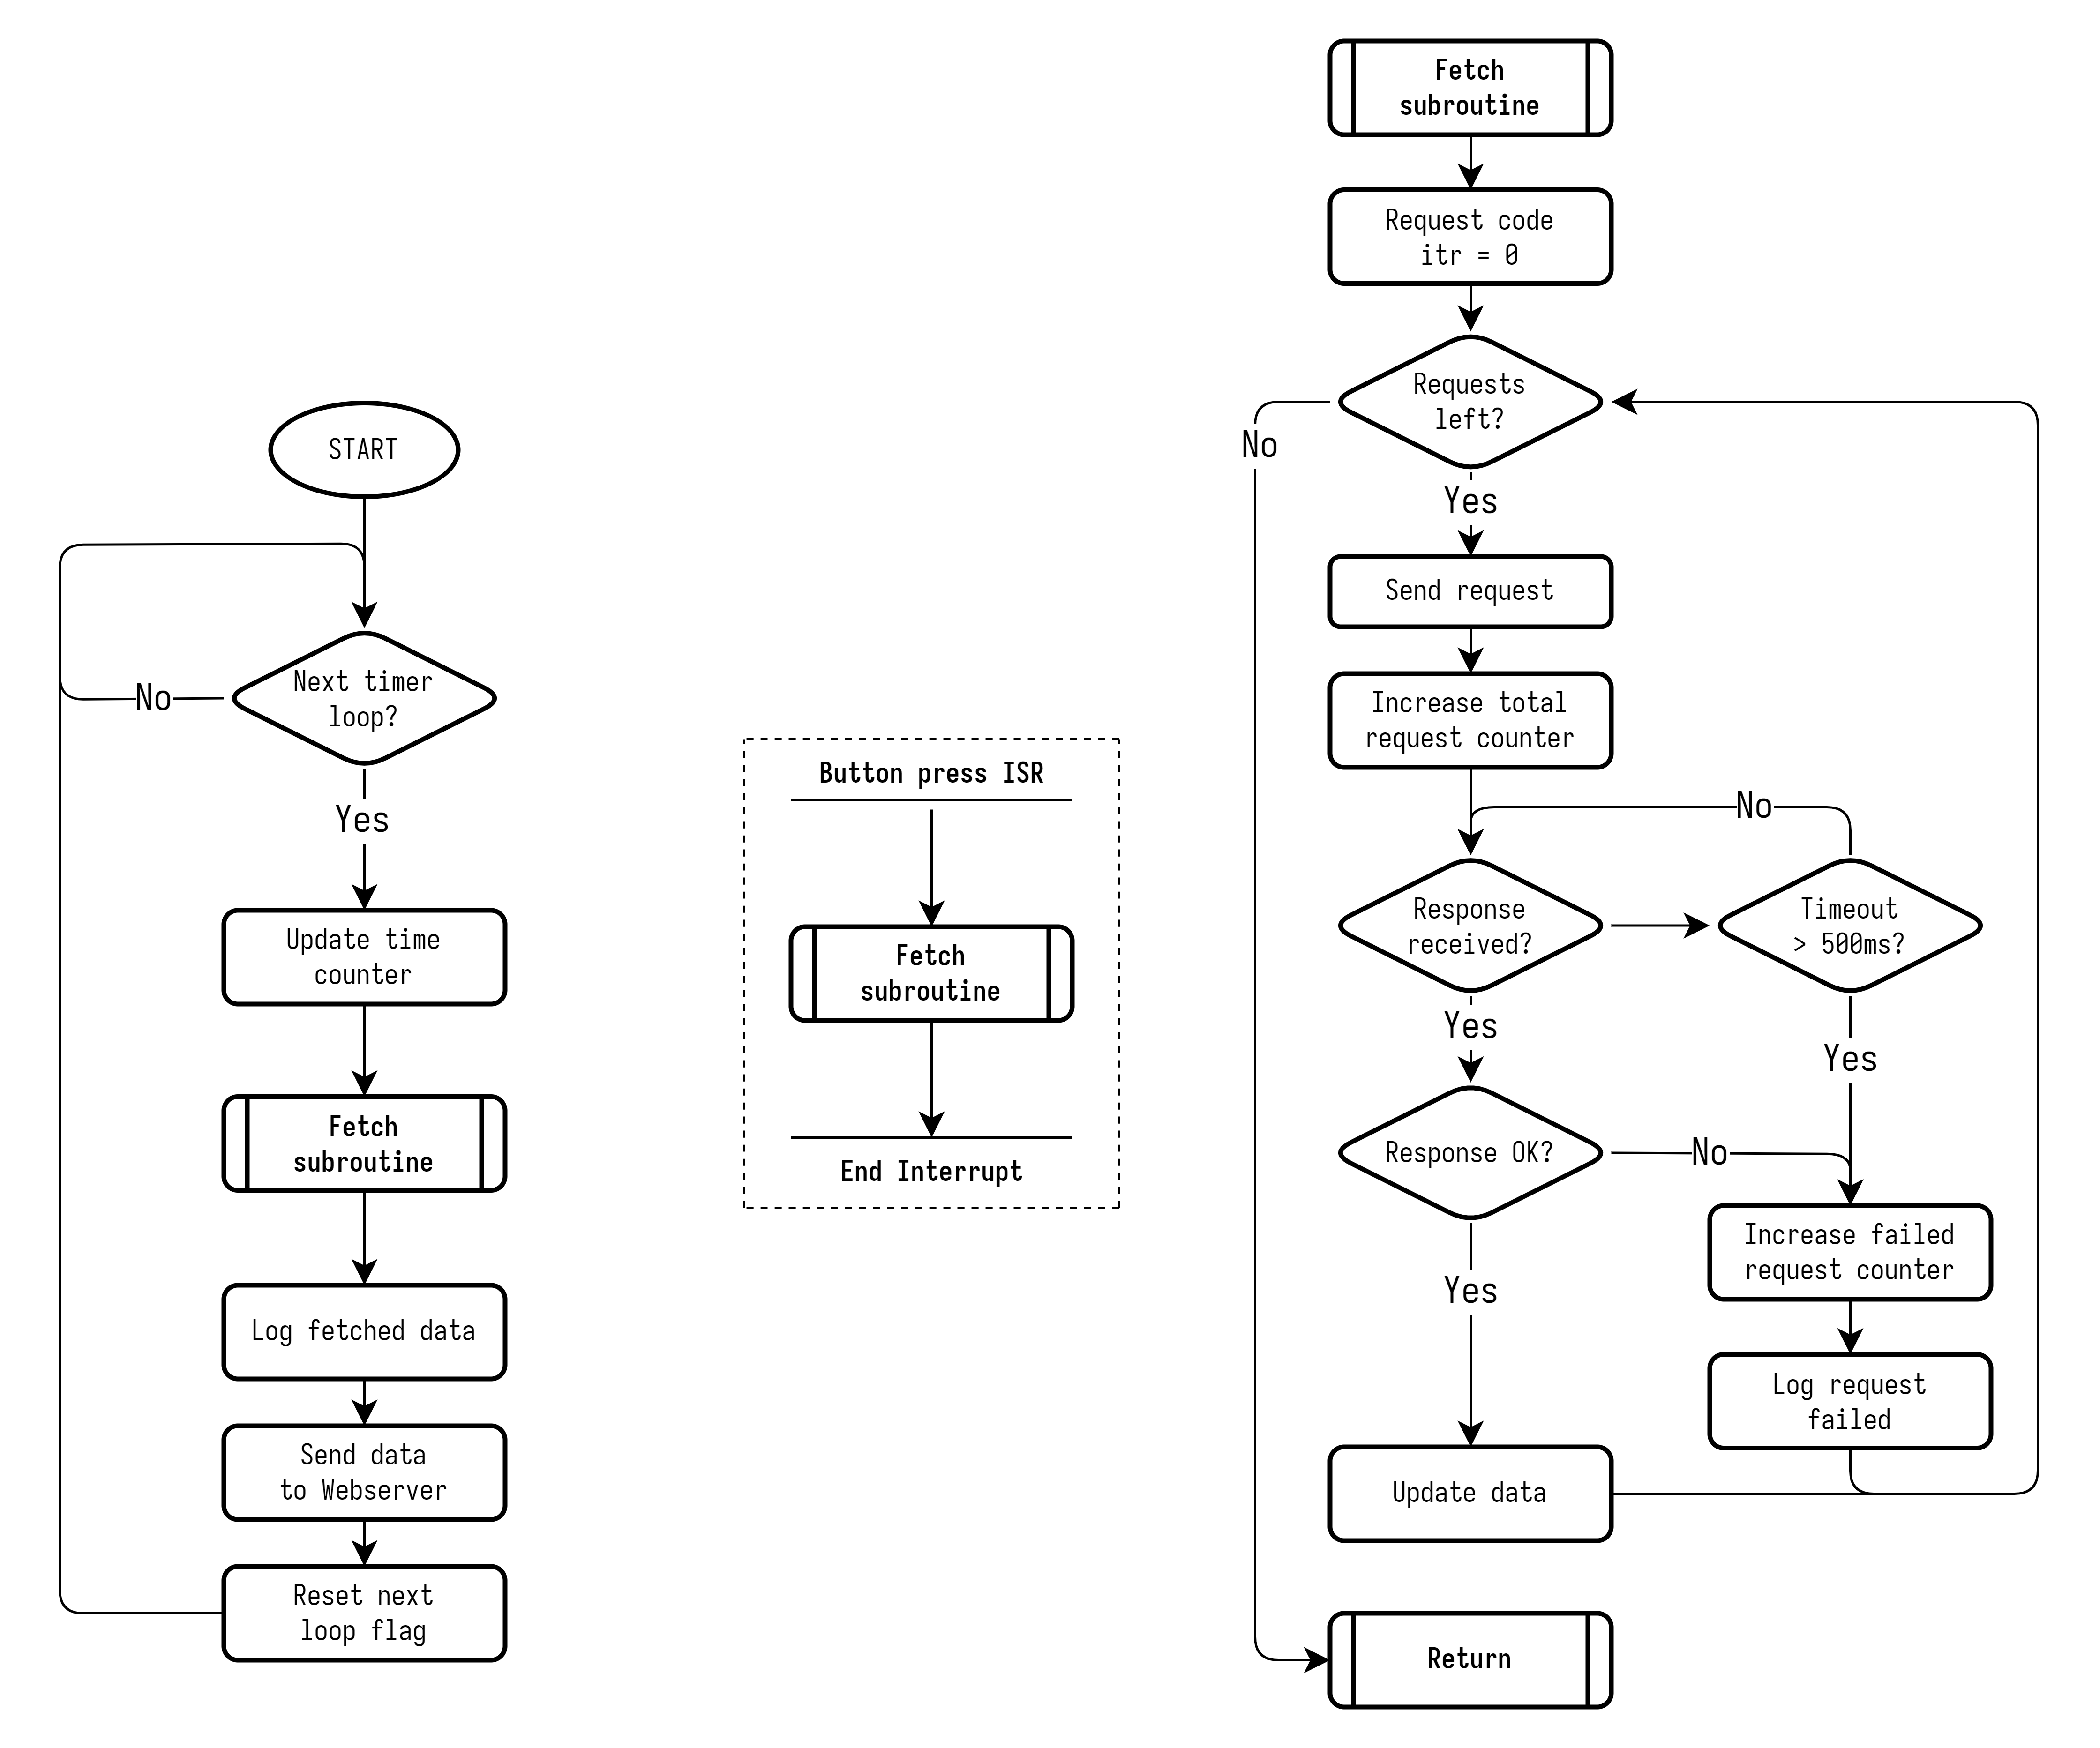
\includegraphics[width=\textwidth]{lora-psn/images/MASTER-loop-flowchart}
    \caption{\label{img:master-flowchart}Schemat blokowy nieskończonej pętli oraz podprogramu zbierania danych
        zaimplementowanych dla modułu MASTER}
\end{figure}

\lstinputlisting[
    language=C++,
    linerange={103-110,112-116},
    caption={Implementacja nieskończonej pętli dla modułu MASTER},
    label={lst:main-loop},
    float=htbp,
]{lora-psn/src/main.cpp}
\lstinputlisting[
    language=C++,
    linerange={133-174},
    caption={Funkcja podprogramu odpowiedzialnego za zbieranie danych w~sieci},
    label={lst:master-fetch},
    float=htbp,
]{lora-psn/src/main.cpp}

Pierwszym elementem podprogramu jest wysłanie nowego zapytania do sieci -- zaimplementowana została do tego funkcja
\texttt{sendRequest()} zawarta w~przestrzeni nazw \texttt{lora}. Jej implementacja przedstawiona została na listingu
\ref{lst:lora-sendrequest}. Pobierany jest kod, który ma zostać wysłany do sieci, następnie, wykorzystując funkcję
\texttt{debug::println()} logowana jest przesyłana wartość. Korzystając z~funkcji, która dostępna jest w~bibliotece do
obsługi modułu rozszerzeń LoRa, wysyłana jest wiadmość do sieci.

\lstinputlisting[
    language=C++,
    linerange={37-43},
    caption={Implementacja funkcji \texttt{lora::sendRequest()}},
    label={lst:lora-sendrequest},
    float=htbp,
]{lora-psn/src/lora.cpp}

Następnie moduł MASTER oczekuje na odpowiedź od modułu SLAVE, który powinien wysłać odpowiedź. Jeżeli odpowiedź zostana
otrzymana w~ciągu 500ms, następuje przejście do sprawdzenia czy pierwsze pole odpowiedzi -- identyfikator -- jest
poprawne. Identyfikator zawiera informację o~ID odpowiadającego SLAVE-a oraz ID danej, której wartość jest przesyłana.
W~przeciwnym razie, na port szeregowy przesyłana jest stosowna informacja, a~licznik zapytań z~błędem odpowiedzi jest
zwiększany. Ostatecznie, jeżeli nie wystapił żaden z~tych błędów, wykorzystując funkcję \texttt{lora::readResponse()},
odczytana zostaje wartość przesłana w~odpowiedzi. Implementacja funkcji odczytującej przedstawiona została na listingu
\ref{lst:lora-readresponse}.

\lstinputlisting[
    language=C++,
    linerange={79-97},
    caption={Implementacja funkcji odczytującej wartość odpowiedzi modułu SLAVE},
    label={lst:lora-readresponse},
    float=htbp,
]{lora-psn/src/lora.cpp}

W~funkcji sprawdzane są ID modułu, który odpowiedź wysłał oraz ID danej. Na podstawie tej wartości, aktualizowana jest
odpowiednia indeks w~tablicy, która odpowiada polu struktury do przechowywania danych odbieranych z~sieci. Struktura ta
przekazywana jest jako referencja do miejsca w~pamięci poprzez wskaźnik do jej adresu.

Ostatnimi elementami każdej iteracji pętli jest przesłanie zebranych danych przez port szeregowy oraz transmisja danych
do modułu pełniącego funkcję serwera sieciowego. Funkcja logowania danych przez port szeregowy została dodana, po to aby
było możliwe debugowanie działania oprogramowania oraz naprawa ewentualnie występujących błędów. Do implementacji
wykorzystana została wykorzystana funkcja szablonowa, która pozwoliła na wykorzytanie tego samego fragmentu kodu do
przesyłania wartości z~tablic o~różnym typie zmiennej (\texttt{float} -- zmiennoprzecinkowa -- dla wartości pochodzących
z~sieci oraz \texttt{int} -- liczby całkowite -- dla wartości związanych ze statystykami zapytań). Na funkcje
wykorzystywane do transmisji danych przez magistralę I2C do modułu serwera sieciowego składa się kod zaimplementowany
korzystając z~tego samego schematu. Przesyłanie wartości z~pojedynczego pola struktury wykorzystuje także funkcję
szablonową, która wywoływana jest kilkukrotnie wewnątrz \texttt{webserverTransmit} w~celu przesłania wszystkich
wymaganych danych. Kod funkcji szablonowych przedstawiony został na listingach \ref{lst:template-log} oraz
\ref{lst:template-transmit}, natomiast implementacja pełnych funkcji do przesyłania danych na listingach
\ref{lst:main-logging} oraz \ref{lst:main-transmitting}. Dodatkowo zaimplementowana została także funkcja pomocniczna do
wyznacznia wartości procentowej zapytań, które zakończyły się błędem. Opiera się ona o~wykonanie dzielenia wartości
z~licznika zapytań z~błędem (\texttt{failedRequests}) przez wartość licznika całkowitej ilości zapytań wysłanych do
każdego z~modułów SLAVE (\texttt{totalRequests}). Kod tej funkcji przedstawiony został na listingu
\ref{lst:main-failedpercent}.

\lstinputlisting[
    language=C++,
    linerange={176-185},
    caption={Implementacja funkcji szablonowej \texttt{logValues()}},
    label={lst:template-log},
    float=htbp,
]{lora-psn/src/main.cpp}

\lstinputlisting[
    language=C++,
    linerange={213-222},
    caption={Implementacja funkcji szablonowej \texttt{transmitPacket()}},
    label={lst:template-transmit},
    float=htbp,
]{lora-psn/src/main.cpp}

\lstinputlisting[
    language=C++,
    linerange={187-211},
    caption={Funkcja wykorzystywana do logowania wartości przez port szeregowy},
    label={lst:main-logging},
    float=htbp,
]{lora-psn/src/main.cpp}

\lstinputlisting[
    language=C++,
    linerange={224-240},
    caption={Funkcja do transmisji danych do modułu serwera przez magistralę I2C},
    label={lst:main-transmitting},
    float=htbp,
]{lora-psn/src/main.cpp}

\lstinputlisting[
    language=C++,
    linerange={242-249},
    caption={Implementacja funkcji pomocnicznej do wyznaczania wartości procentowej zapytań z~błędem},
    label={lst:main-failedpercent},
    float=htbp,
]{lora-psn/src/main.cpp}

\FloatBarrier
\subsection{Oprogramowanie modułów SLAVE\label{sect:firmware-slave}} W~przypadku modułów SLAVE działanie kodu
w~nieskończonej pętli zostało zaimplementowane inaczej. Poza wykonywaniem zadań bazując na zegarze, w~tym przypadku
z~okresem 5~sekund,

\FloatBarrier
\section{Implementacja oprogramowania modułu serwera sieciowego\label{sect:firmware-webserver}}